\documentclass[11pt]{book}

\setcounter{chapter}{3}
\newcommand{\docclass}{CSC 341 (20sp)}
\newcommand{\doctitle}{Deterministic Finite Automata}
\newcommand{\docauthor}{Peter-Michael Osera}

\usepackage{reading}

\begin{document}

\begin{center}
  (Turn-in problems are indicated with a dagger \turninproblem{}.)
\end{center}

\begin{center}
  \large\textbf{{\doctitle}}
\end{center}

\vspace{2em}

%%%%%%%%%%%%%%%%%%%%%%%%%%%%%%%%%%%%%%%%%%%%%%%%%%%%%%%%%%%%%%%%%%%%%%%%%%%%%%%%

\begin{problem}{Complicating the Process}

On your own, come up a complicated \emph{non-deterministic finite automata} with
at most \emph{8 states} for your peers to analyze.  Think carefully about what
makes a NFA more complicated than a DFA and any particularly nasty corner cases
about its definition that you think might trick your peers.

Draw a diagram of the NFA in the space below and verify its language.  You will
exchange NFAs with a partner and try to derive your partner's NFA's language.

\end{problem}

\newpage

%%%%%%%%%%%%%%%%%%%%%%%%%%%%%%%%%%%%%%%%%%%%%%%%%%%%%%%%%%%%%%%%%%%%%%%%%%%%%%%%

\begin{problem}{Interpretation}

\begin{center}
  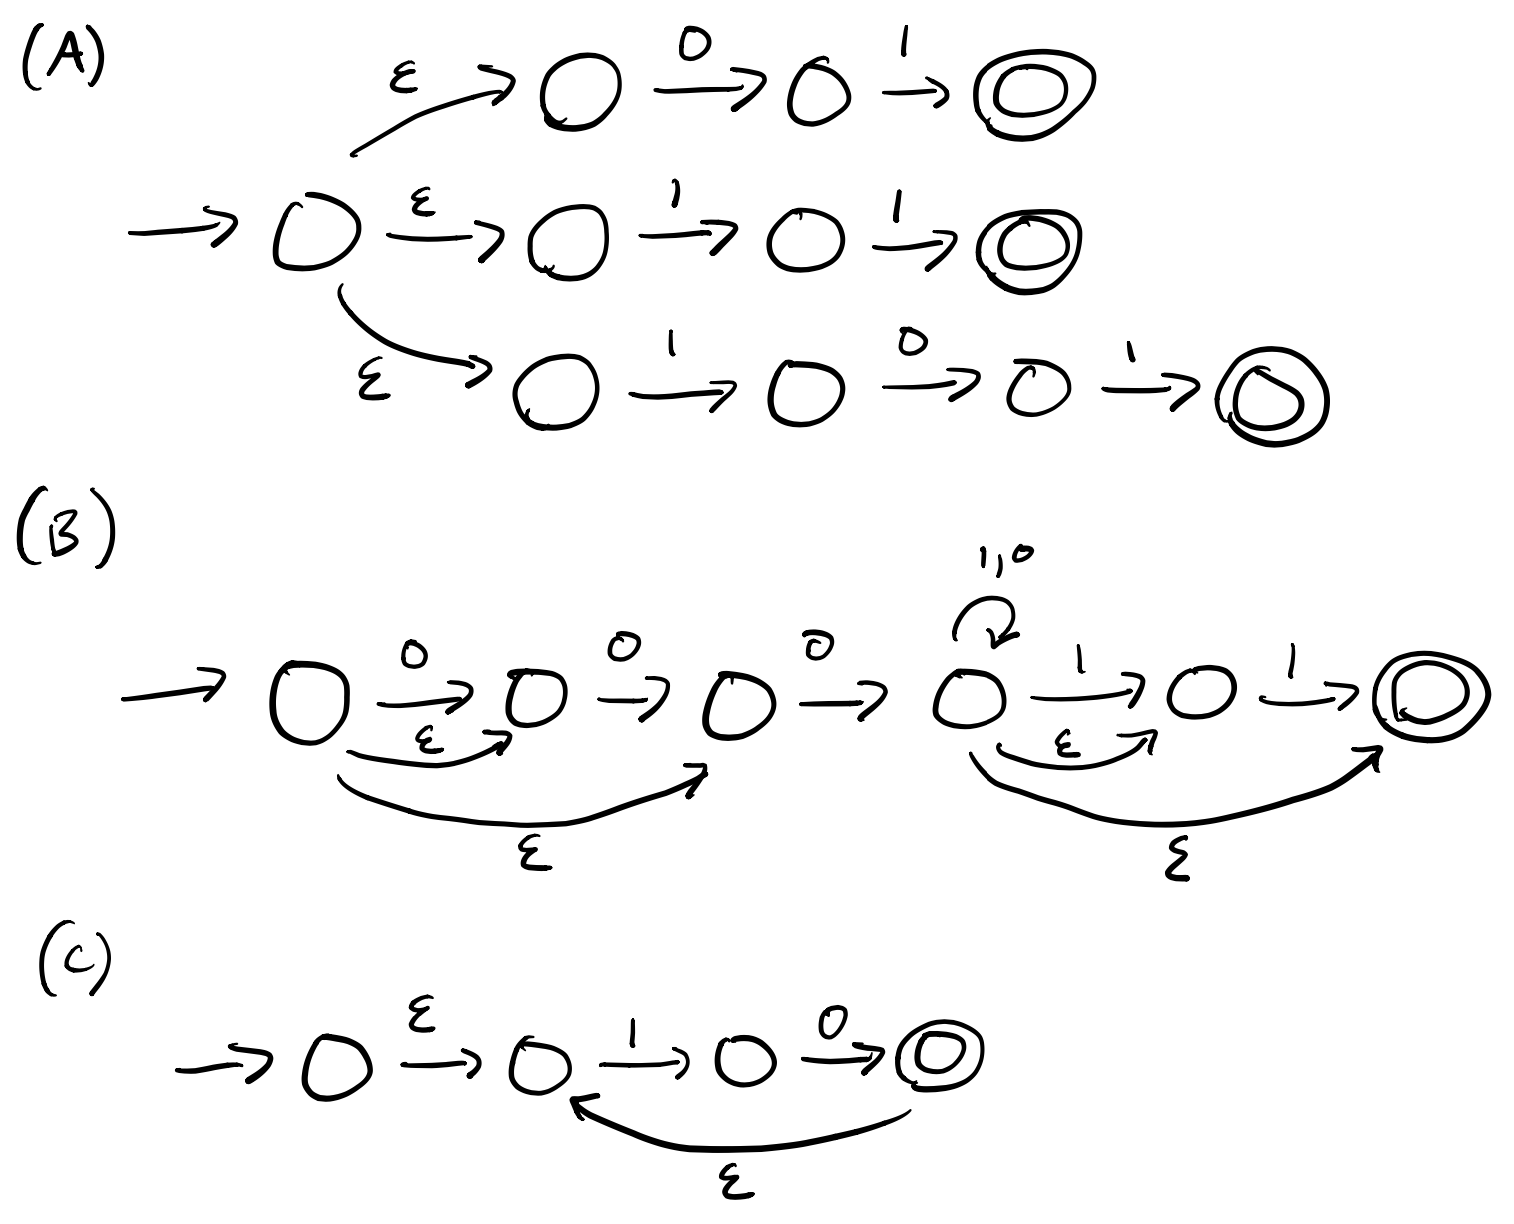
\includegraphics[width=\textwidth]{nfas}
\end{center}

\noindent (a) Determine whether the strings:
\begin{itemize}
  \item 101
  \item 0111
  \item 1010
  \item \( \epsilon \)
\end{itemize}
are accepted by the NFAs above.

\vspace{1em}

\noindent (b) \turninproblem{} Give a formal description of the languages that
each of the NFAs above recognize.

\end{problem}

\end{document}
